%% LyX 2.4.4 created this file.  For more info, see https://www.lyx.org/.
%% Do not edit unless you really know what you are doing.
\documentclass[english]{article}
\usepackage[T1]{fontenc}
\usepackage[latin9]{inputenc}
\usepackage{enumitem}
\usepackage{amsmath}
\usepackage{amsthm}
\usepackage{graphicx}
\usepackage{geometry}
\geometry{verbose,tmargin=1in,bmargin=1in,lmargin=1in,rmargin=1in}
\usepackage{setspace}
\onehalfspacing

\makeatletter
%%%%%%%%%%%%%%%%%%%%%%%%%%%%%% Textclass specific LaTeX commands.
\newlength{\lyxlabelwidth}      % auxiliary length 
\numberwithin{equation}{section}
\numberwithin{figure}{section}

%%%%%%%%%%%%%%%%%%%%%%%%%%%%%% User specified LaTeX commands.
\usepackage{fancyhdr}
\usepackage{lastpage}
\pagestyle{fancy}
\usepackage{enumitem}
\usepackage{ifthen}
\usepackage{multicol}

\DeclareMathSizes{10}{10}{10}{10}

\usepackage{tikz}
\usetikzlibrary{patterns}
\usetikzlibrary{plotmarks}
\usepackage{pgfplots}
\pgfplotsset{compat=newest}

\usepackage{advdate}    % Advancing/saving dates
\usepackage{datetime}   % Dates formatting
\usepackage{datenumber} % Counters for dates
\usdate
% Added by lyx2lyx
\setlength{\parskip}{\smallskipamount}
\setlength{\parindent}{0pt}

\makeatother

\usepackage{babel}
\begin{document}
\renewcommand{\author}{Dr.\,James Ashe}

\newcommand{\classNum}{232}

\newcommand{\classSec}{}

\newcommand{\examType}{Table of Formulas}

\renewcommand{\date}{}

%%First page's header%%%%%%%%%%%%%%%%%%%%%%
\fancypagestyle{firststyle} %%header settings for first pagr
{
	\fancyhead[L]{MTH \classNum{}(\classSec{}) \author{}\\
	\textbf{\examType{}} \date{}}
	\fancyhead[C]{\textbf{}}
	\setlength{\headsep}{20pt}
}
%%%%%%%%%%%%%%%%%%%%%%%%%%%%%%%%%%%%%%%%%%

%%Next page's header%%%%%%%%%%%%%%%%%%%%%%%
\setlist{nolistsep}
\lhead{MTH \classNum{}(\classSec{})} 
\chead{\textbf{}} 
\cfoot{\thepage{}~of~\pageref{LastPage}} 
\setlength{\headsep}{5pt} 
%%%%%%%%%%%%%%%%%%%%%%%%%%%%%%%%%%%%%%%%%%%

%%Various settings; see the preamble for other settings%%%%%
%\setenumerate[0]{leftmargin=12pt,itemindent=0pt,labelwidth=0pt}
\setenumerate[0]{itemsep=6pt}
\renewcommand{\labelenumi}{\textbf{\arabic{enumi}.}}
\renewcommand{\labelenumii}{\textbf{\alph{enumii}.}}
\thispagestyle{firststyle} %%sets first page style so that it has differeny heading
%%%%%%%%%%%%%%%%%%%%%%%%%%%%%%%%%%%%%%%%%%

\begin{multicols}{2}

\subsubsection*{Formulas for Derivatives}
\begin{enumerate}
\item $\frac{d}{dx}\left(x^{n}\right)=nx^{n-1}$
\item $\frac{d}{dx}\left[f\left(g(x)\right)\right]=f'\left(g(x)\right)\cdot g'(x)$
(Chain rule)
\item $\frac{d}{dx}\left(f(x)g(x)\right)=f'(x)g(x)+f(x)g'(x)$
\item $\frac{d}{dx}\left(\frac{f(x)}{g(x)}\right)=\frac{g(x)f'(x)-f(x)g'(x)}{\left(g(x)\right)^{2}}$
\item $\frac{d}{dx}(\sin ax)=a\cos ax$
\item $\frac{d}{dx}(\cos ax)=-a\sin a$
\item $\frac{d}{dx}e^{x}=e^{x}$
\item $\frac{d}{dx}e^{u(x)}=u'(x)e^{u(x)}$
\item $\frac{d}{dx}\left(b^{x}\right)=b^{x}\ln b$
\item $\frac{d}{dx}\left(b^{u(x)}\right)=b^{u(x)}\left(\ln b\right)u'(x)$
\item $\frac{d}{dx}\ln x=\frac{1}{x}$
\item $\frac{d}{dx}\left(\log_{b}x\right)=\frac{1}{x\ln b}$, for $x>0$\columnbreak
\end{enumerate}

\subsubsection*{Formulas for Integration}
\begin{enumerate}
\item $\int x^{n}\,dx=\frac{1}{n+1}x^{n+1}+C$; $n\neq-1$
\item $\int\cos ax\,dx=\frac{1}{a}\sin ax+C$
\item $\int\sin ax\,dx=-\frac{1}{a}\cos ax+C$
\item $\int e^{ax}\,dx=\frac{1}{a}e^{ax}+C$
\item $\int\frac{1}{x}\,dx=\ln\left|x\right|+C$
\item $\int b^{x}\,dx=\frac{1}{\ln b}b^{x}+C$ for $b>0$ and $b\neq1$
\item $\int\ln x\,dx=x\ln x-x+C$
\item $\int\tan x\,dx=\ln\left|\cos x\right|+C$
\item $\int\sec x\,dx=\ln\left|\sec x+\tan x\right|+C$
\item $\int f(g(x))g'(x)\,dx=\int f(u)\,du$ (Substitution rule)
\item $\int u\,dv=uv-\int v\,du$ (Integration by parts)
\end{enumerate}
\end{multicols}

\begin{multicols}{2}

\textbf{Trigonometric Substitution Identities}
\begin{enumerate}
\item $a^{2}-x^{2}\rightarrow a^{2}\cos^{2}\theta$ where $x=a\sin\theta$
\item $a^{2}+x^{2}\rightarrow a^{2}\sec^{2}\theta$ where $x=a\sin\theta$
\item $x^{2}-a^{2}\rightarrow a^{2}\tan^{2}\theta$ where $x=a\sec\theta$
\end{enumerate}
\textbf{Pythagorean Identity}
\begin{enumerate}[resume]
\item $\sin^{2}\theta+\cos^{2}\theta=1$
\end{enumerate}
\textbf{Half-Angle Formulas }
\begin{enumerate}[resume]
\item $\cos^{2}\theta=\frac{1+\cos2\theta}{2}$; ~~$\sin^{2}\theta=\frac{1-\cos2\theta}{2}$
\end{enumerate}
\textbf{Double-Angle Identities}
\begin{enumerate}[resume]
\item $\sin2\theta=2\sin\theta\cos\theta$;~~$\cos2\theta=2\cos^{2}\theta-1$
\end{enumerate}
\center{\includegraphics[width=4cm]{D:/home/jim/JamesAshe/JCSU/Calc_2_MTH_232/images/Trig_Sub_reference_Triangle_a^2-x^2.png}}\columnbreak\footnotesize

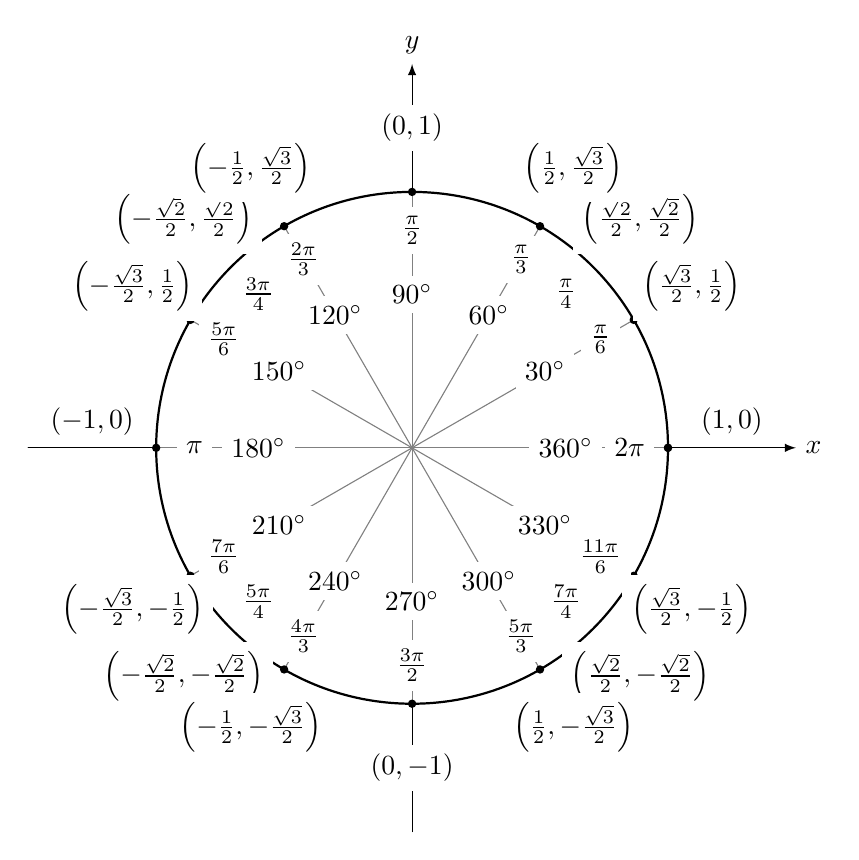
\begin{tikzpicture}[scale=3.25,cap=round,>=latex]         %scale=5,3 % draw the coordinates         
	\draw[->] (-1.5cm,0cm) -- (1.5cm,0cm) node[right,fill=white] {$x$};         
	\draw[->] (0cm,-1.5cm) -- (0cm,1.5cm) node[above,fill=white] {$y$};
        % draw the unit circle         
	\draw[thick] (0cm,0cm) circle(1cm);
    \foreach \x in {0,30,...,360} {                 % lines from center to point                 
			\draw[gray] (0cm,0cm) -- (\x:1cm);                 % dots at each point                 
			\filldraw[black] (\x:1cm) circle(0.4pt);                 % draw each angle in degrees                 
			\draw (\x:0.6cm) node[fill=white] {$\x^\circ$};         
			}
        % draw each angle in radians         
	\foreach \x/\xtext in {
		30/\frac{\pi}{6},             
		45/\frac{\pi}{4},             
		60/\frac{\pi}{3},             			
		90/\frac{\pi}{2},             
		120/\frac{2\pi}{3},             
		135/\frac{3\pi}{4},             
		150/\frac{5\pi}{6},             
		180/\pi,             	
		210/\frac{7\pi}{6},             
		225/\frac{5\pi}{4},             
		240/\frac{4\pi}{3},             
		270/\frac{3\pi}{2},             			
		300/\frac{5\pi}{3},             		
		315/\frac{7\pi}{4},            
		330/\frac{11\pi}{6},             
		360/2\pi}                 
			\draw (\x:0.85cm) node[fill=white] {$\xtext$};
	\foreach \x/\xtext/\y in {             % the coordinates for the first quadrant             
		30/\frac{\sqrt{3}}{2}/\frac{1}{2},             			
		45/\frac{\sqrt{2}}{2}/\frac{\sqrt{2}}{2},             
		60/\frac{1}{2}/\frac{\sqrt{3}}{2},             % the coordinates for the second quadrant             
		150/-\frac{\sqrt{3}}{2}/\frac{1}{2},             
		135/-\frac{\sqrt{2}}{2}/\frac{\sqrt{2}}{2},             			
		120/-\frac{1}{2}/\frac{\sqrt{3}}{2},             % the coordinates for the third quadrant             
		210/-\frac{\sqrt{3}}{2}/-\frac{1}{2},             
		225/-\frac{\sqrt{2}}{2}/-\frac{\sqrt{2}}{2},             
		240/-\frac{1}{2}/-\frac{\sqrt{3}}{2},             % the coordinates for the fourth quadrant             
		330/\frac{\sqrt{3}}{2}/-\frac{1}{2},             				
		315/\frac{\sqrt{2}}{2}/-\frac{\sqrt{2}}{2},             
		300/\frac{1}{2}/-\frac{\sqrt{3}}{2}}                 
			\draw (\x:1.261cm) node[fill=white] {$\left(\xtext,\y\right)$};
        % draw the horizontal and vertical coordinates         % the placement is better this way         
	\draw (-1.25cm,0cm) node[above=1pt] {$(-1,0)$}               
		  (1.25cm,0cm)  node[above=1pt] {$(1,0)$}               
		  (0cm,-1.25cm) node[fill=white] {$(0,-1)$}               
          (0cm,1.25cm)  node[fill=white] {$(0,1)$};     
\end{tikzpicture}

\end{multicols}
\end{document}
